\documentclass[twoside]{book}

% Packages required by doxygen
\usepackage{fixltx2e}
\usepackage{calc}
\usepackage{doxygen}
\usepackage[export]{adjustbox} % also loads graphicx
\usepackage{graphicx}
\usepackage[utf8]{inputenc}
\usepackage{makeidx}
\usepackage{multicol}
\usepackage{multirow}
\PassOptionsToPackage{warn}{textcomp}
\usepackage{textcomp}
\usepackage[nointegrals]{wasysym}
\usepackage[table]{xcolor}

% NLS support packages
\usepackage[brazil]{babel}
% Font selection
\usepackage[T1]{fontenc}
\usepackage[scaled=.90]{helvet}
\usepackage{courier}
\usepackage{amssymb}
\usepackage{sectsty}
\renewcommand{\familydefault}{\sfdefault}
\allsectionsfont{%
  \fontseries{bc}\selectfont%
  \color{darkgray}%
}
\renewcommand{\DoxyLabelFont}{%
  \fontseries{bc}\selectfont%
  \color{darkgray}%
}
\newcommand{\+}{\discretionary{\mbox{\scriptsize$\hookleftarrow$}}{}{}}

% Page & text layout
\usepackage{geometry}
\geometry{%
  a4paper,%
  top=2.5cm,%
  bottom=2.5cm,%
  left=2.5cm,%
  right=2.5cm%
}
\tolerance=750
\hfuzz=15pt
\hbadness=750
\setlength{\emergencystretch}{15pt}
\setlength{\parindent}{0cm}
\setlength{\parskip}{3ex plus 2ex minus 2ex}
\makeatletter
\renewcommand{\paragraph}{%
  \@startsection{paragraph}{4}{0ex}{-1.0ex}{1.0ex}{%
    \normalfont\normalsize\bfseries\SS@parafont%
  }%
}
\renewcommand{\subparagraph}{%
  \@startsection{subparagraph}{5}{0ex}{-1.0ex}{1.0ex}{%
    \normalfont\normalsize\bfseries\SS@subparafont%
  }%
}
\makeatother

% Headers & footers
\usepackage{fancyhdr}
\pagestyle{fancyplain}
\fancyhead[LE]{\fancyplain{}{\bfseries\thepage}}
\fancyhead[CE]{\fancyplain{}{}}
\fancyhead[RE]{\fancyplain{}{\bfseries\leftmark}}
\fancyhead[LO]{\fancyplain{}{\bfseries\rightmark}}
\fancyhead[CO]{\fancyplain{}{}}
\fancyhead[RO]{\fancyplain{}{\bfseries\thepage}}
\fancyfoot[LE]{\fancyplain{}{}}
\fancyfoot[CE]{\fancyplain{}{}}
\fancyfoot[RE]{\fancyplain{}{\bfseries\scriptsize Gerado por Doxygen }}
\fancyfoot[LO]{\fancyplain{}{\bfseries\scriptsize Gerado por Doxygen }}
\fancyfoot[CO]{\fancyplain{}{}}
\fancyfoot[RO]{\fancyplain{}{}}
\renewcommand{\footrulewidth}{0.4pt}
\renewcommand{\chaptermark}[1]{%
  \markboth{#1}{}%
}
\renewcommand{\sectionmark}[1]{%
  \markright{\thesection\ #1}%
}

% Indices & bibliography
\usepackage{natbib}
\usepackage[titles]{tocloft}
\setcounter{tocdepth}{3}
\setcounter{secnumdepth}{5}
\makeindex

% Hyperlinks (required, but should be loaded last)
\usepackage{ifpdf}
\ifpdf
  \usepackage[pdftex,pagebackref=true]{hyperref}
\else
  \usepackage[ps2pdf,pagebackref=true]{hyperref}
\fi
\hypersetup{%
  colorlinks=true,%
  linkcolor=blue,%
  citecolor=blue,%
  unicode%
}

% Custom commands
\newcommand{\clearemptydoublepage}{%
  \newpage{\pagestyle{empty}\cleardoublepage}%
}

\usepackage{caption}
\captionsetup{labelsep=space,justification=centering,font={bf},singlelinecheck=off,skip=4pt,position=top}

%===== C O N T E N T S =====

\begin{document}

% Titlepage & ToC
\hypersetup{pageanchor=false,
             bookmarksnumbered=true,
             pdfencoding=unicode
            }
\pagenumbering{alph}
\begin{titlepage}
\vspace*{7cm}
\begin{center}%
{\Large My Project }\\
\vspace*{1cm}
{\large Gerado por Doxygen 1.8.14}\\
\end{center}
\end{titlepage}
\clearemptydoublepage
\pagenumbering{roman}
\tableofcontents
\clearemptydoublepage
\pagenumbering{arabic}
\hypersetup{pageanchor=true}

%--- Begin generated contents ---
\chapter{Índice Hierárquico}
\section{Class Hierarchy}
This inheritance list is sorted roughly, but not completely, alphabetically\+:\begin{DoxyCompactList}
\item \contentsline{section}{com.\+company.\+Main}{\pageref{classcom_1_1company_1_1_main}}{}
\item \contentsline{section}{com.\+company.\+Mundo}{\pageref{classcom_1_1company_1_1_mundo}}{}
\item \contentsline{section}{com.\+company.\+Veiculo}{\pageref{classcom_1_1company_1_1_veiculo}}{}
\begin{DoxyCompactList}
\item \contentsline{section}{com.\+company.\+Caminhao}{\pageref{classcom_1_1company_1_1_caminhao}}{}
\item \contentsline{section}{com.\+company.\+Carro}{\pageref{classcom_1_1company_1_1_carro}}{}
\item \contentsline{section}{com.\+company.\+Moto}{\pageref{classcom_1_1company_1_1_moto}}{}
\end{DoxyCompactList}
\end{DoxyCompactList}

\chapter{Índice dos Componentes}
\section{Lista de Classes}
Aqui estão as classes, estruturas, uniões e interfaces e suas respectivas descrições\+:\begin{DoxyCompactList}
\item\contentsline{section}{\mbox{\hyperlink{classcom_1_1company_1_1_caminhao}{com.\+company.\+Caminhao}} }{\pageref{classcom_1_1company_1_1_caminhao}}{}
\item\contentsline{section}{\mbox{\hyperlink{classcom_1_1company_1_1_carro}{com.\+company.\+Carro}} }{\pageref{classcom_1_1company_1_1_carro}}{}
\item\contentsline{section}{\mbox{\hyperlink{classcom_1_1company_1_1_main}{com.\+company.\+Main}} }{\pageref{classcom_1_1company_1_1_main}}{}
\item\contentsline{section}{\mbox{\hyperlink{classcom_1_1company_1_1_moto}{com.\+company.\+Moto}} }{\pageref{classcom_1_1company_1_1_moto}}{}
\item\contentsline{section}{\mbox{\hyperlink{classcom_1_1company_1_1_mundo}{com.\+company.\+Mundo}} }{\pageref{classcom_1_1company_1_1_mundo}}{}
\item\contentsline{section}{\mbox{\hyperlink{classcom_1_1company_1_1_veiculo}{com.\+company.\+Veiculo}} }{\pageref{classcom_1_1company_1_1_veiculo}}{}
\end{DoxyCompactList}

\chapter{Classes}
\hypertarget{classcom_1_1company_1_1_caminhao}{}\section{com.\+company.\+Caminhao Class Reference}
\label{classcom_1_1company_1_1_caminhao}\index{com.\+company.\+Caminhao@{com.\+company.\+Caminhao}}
Inheritance diagram for com.\+company.\+Caminhao\+:\begin{figure}[H]
\begin{center}
\leavevmode
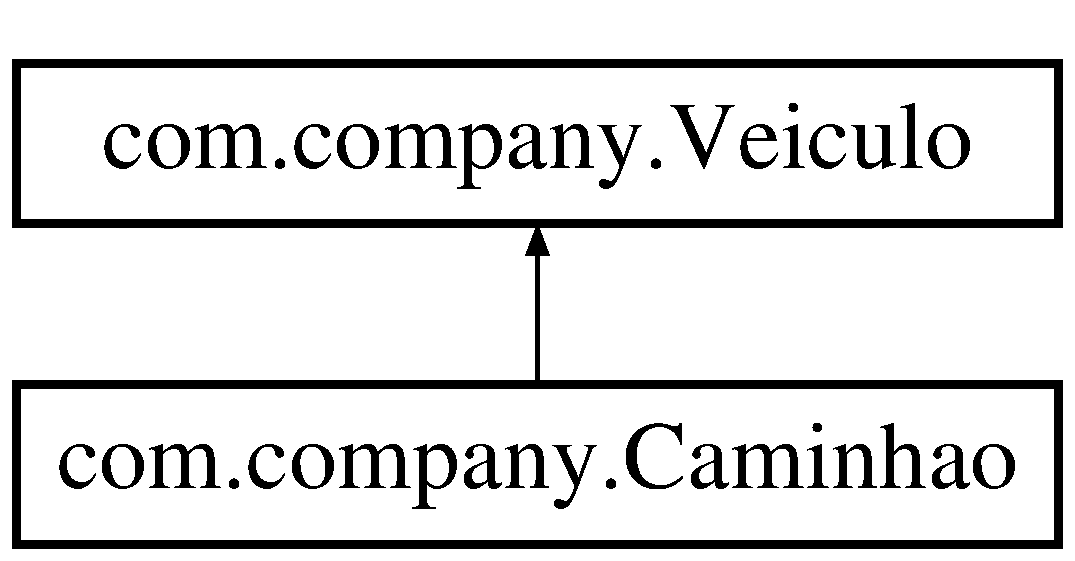
\includegraphics[height=2.000000cm]{classcom_1_1company_1_1_caminhao}
\end{center}
\end{figure}
\subsection*{Public Member Functions}
\begin{DoxyCompactItemize}
\item 
\mbox{\Hypertarget{classcom_1_1company_1_1_caminhao_ae170d22b1de70887d19e62b1c5bf9c13}\label{classcom_1_1company_1_1_caminhao_ae170d22b1de70887d19e62b1c5bf9c13}} 
{\bfseries Caminhao} (int x, int y)
\item 
\mbox{\Hypertarget{classcom_1_1company_1_1_caminhao_acee8e3ca4f4c8659fdfc8bfb527a3273}\label{classcom_1_1company_1_1_caminhao_acee8e3ca4f4c8659fdfc8bfb527a3273}} 
void \mbox{\hyperlink{classcom_1_1company_1_1_caminhao_acee8e3ca4f4c8659fdfc8bfb527a3273}{move}} (\mbox{\hyperlink{classcom_1_1company_1_1_caminhao}{Caminhao}} a)
\begin{DoxyCompactList}\small\item\em logica para o caminhao se mover no mapa \end{DoxyCompactList}\end{DoxyCompactItemize}


The documentation for this class was generated from the following file\+:\begin{DoxyCompactItemize}
\item 
Caminhao.\+java\end{DoxyCompactItemize}

\hypertarget{classcom_1_1company_1_1_carro}{}\section{com.\+company.\+Carro Class Reference}
\label{classcom_1_1company_1_1_carro}\index{com.\+company.\+Carro@{com.\+company.\+Carro}}
Inheritance diagram for com.\+company.\+Carro\+:\begin{figure}[H]
\begin{center}
\leavevmode
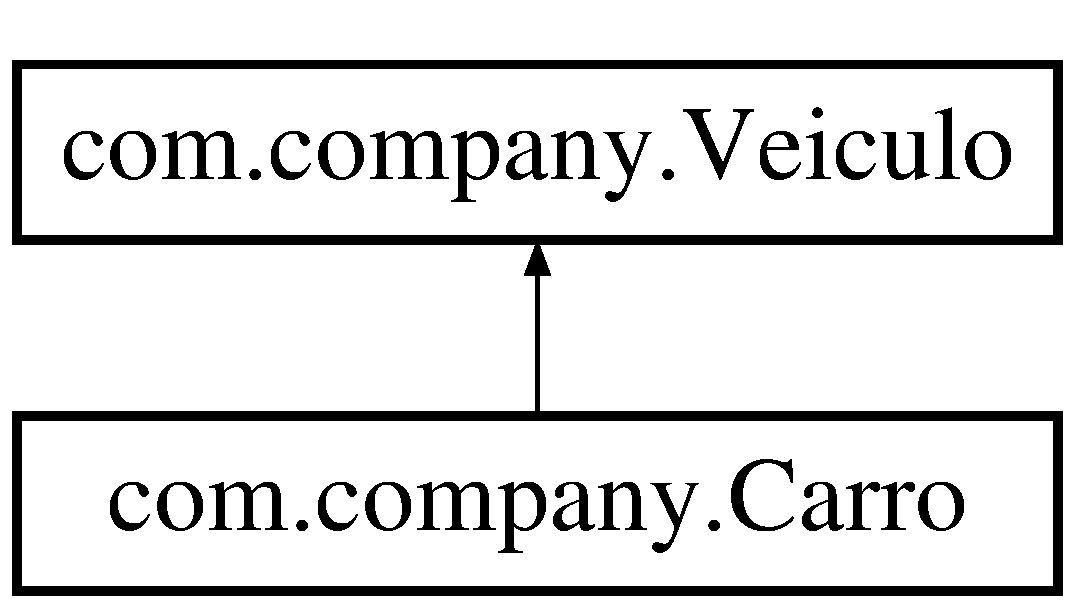
\includegraphics[height=2.000000cm]{classcom_1_1company_1_1_carro}
\end{center}
\end{figure}
\subsection*{Public Member Functions}
\begin{DoxyCompactItemize}
\item 
\mbox{\Hypertarget{classcom_1_1company_1_1_carro_a37f52c32727826ff07e5daf63f9079ef}\label{classcom_1_1company_1_1_carro_a37f52c32727826ff07e5daf63f9079ef}} 
{\bfseries Carro} (int x, int y)
\item 
\mbox{\Hypertarget{classcom_1_1company_1_1_carro_aa768871c4c1c6514f123442ee55915f8}\label{classcom_1_1company_1_1_carro_aa768871c4c1c6514f123442ee55915f8}} 
void \mbox{\hyperlink{classcom_1_1company_1_1_carro_aa768871c4c1c6514f123442ee55915f8}{move}} (\mbox{\hyperlink{classcom_1_1company_1_1_carro}{Carro}} a)
\begin{DoxyCompactList}\small\item\em logica para o carro se mover no mapa \end{DoxyCompactList}\end{DoxyCompactItemize}


The documentation for this class was generated from the following file\+:\begin{DoxyCompactItemize}
\item 
Carro.\+java\end{DoxyCompactItemize}

\hypertarget{classcom_1_1company_1_1_main}{}\section{Referência da Classe com.\+company.\+Main}
\label{classcom_1_1company_1_1_main}\index{com.\+company.\+Main@{com.\+company.\+Main}}
\subsection*{Membros Públicos Estáticos}
\begin{DoxyCompactItemize}
\item 
static void \mbox{\hyperlink{classcom_1_1company_1_1_main_a6bc3d68479e38e54554042566ab5e157}{main}} (String\mbox{[}$\,$\mbox{]} args)
\end{DoxyCompactItemize}


\subsection{Funções membros}
\mbox{\Hypertarget{classcom_1_1company_1_1_main_a6bc3d68479e38e54554042566ab5e157}\label{classcom_1_1company_1_1_main_a6bc3d68479e38e54554042566ab5e157}} 
\index{com\+::company\+::\+Main@{com\+::company\+::\+Main}!main@{main}}
\index{main@{main}!com\+::company\+::\+Main@{com\+::company\+::\+Main}}
\subsubsection{\texorpdfstring{main()}{main()}}
{\footnotesize\ttfamily static void com.\+company.\+Main.\+main (\begin{DoxyParamCaption}\item[{String \mbox{[}$\,$\mbox{]}}]{args }\end{DoxyParamCaption})\hspace{0.3cm}{\ttfamily [inline]}, {\ttfamily [static]}}

um loop infinito

da um tempo para acontecer o loop 

A documentação para essa classe foi gerada a partir do seguinte arquivo\+:\begin{DoxyCompactItemize}
\item 
Main.\+java\end{DoxyCompactItemize}

\hypertarget{classcom_1_1company_1_1_moto}{}\section{Referência da Classe com.\+company.\+Moto}
\label{classcom_1_1company_1_1_moto}\index{com.\+company.\+Moto@{com.\+company.\+Moto}}
Diagrama de hierarquia para com.\+company.\+Moto\+:\begin{figure}[H]
\begin{center}
\leavevmode
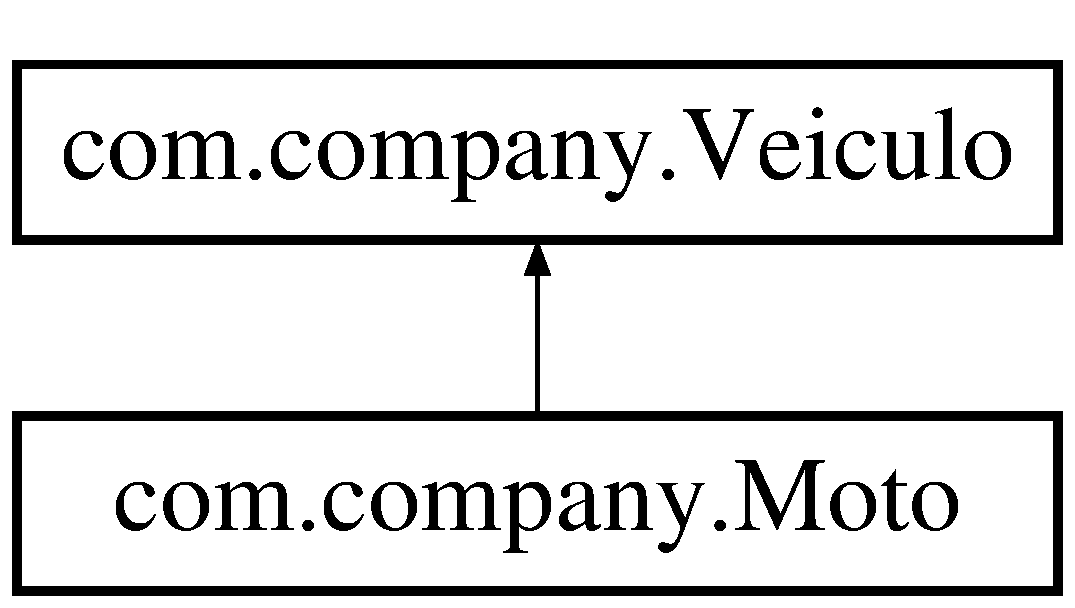
\includegraphics[height=2.000000cm]{classcom_1_1company_1_1_moto}
\end{center}
\end{figure}
\subsection*{Membros Públicos}
\begin{DoxyCompactItemize}
\item 
\mbox{\Hypertarget{classcom_1_1company_1_1_moto_a515d5ceb54df30829f64bec34f052d38}\label{classcom_1_1company_1_1_moto_a515d5ceb54df30829f64bec34f052d38}} 
{\bfseries Moto} (int x, int y)
\item 
\mbox{\Hypertarget{classcom_1_1company_1_1_moto_a6dd391cc77dd0cac8fc670a5b93e4b0d}\label{classcom_1_1company_1_1_moto_a6dd391cc77dd0cac8fc670a5b93e4b0d}} 
void \mbox{\hyperlink{classcom_1_1company_1_1_moto_a6dd391cc77dd0cac8fc670a5b93e4b0d}{move}} (\mbox{\hyperlink{classcom_1_1company_1_1_moto}{Moto}} a)
\begin{DoxyCompactList}\small\item\em logica para a moto se mover no mapa \end{DoxyCompactList}\end{DoxyCompactItemize}


A documentação para essa classe foi gerada a partir do seguinte arquivo\+:\begin{DoxyCompactItemize}
\item 
Moto.\+java\end{DoxyCompactItemize}

\hypertarget{classcom_1_1company_1_1_mundo}{}\section{Referência da Classe com.\+company.\+Mundo}
\label{classcom_1_1company_1_1_mundo}\index{com.\+company.\+Mundo@{com.\+company.\+Mundo}}
\subsection*{Membros Públicos}
\begin{DoxyCompactItemize}
\item 
\mbox{\Hypertarget{classcom_1_1company_1_1_mundo_a4a84d2b83fe16d469f53c5722b185f51}\label{classcom_1_1company_1_1_mundo_a4a84d2b83fe16d469f53c5722b185f51}} 
void \mbox{\hyperlink{classcom_1_1company_1_1_mundo_a4a84d2b83fe16d469f53c5722b185f51}{start}} ()
\begin{DoxyCompactList}\small\item\em é executado no loop do main. \end{DoxyCompactList}\item 
\mbox{\Hypertarget{classcom_1_1company_1_1_mundo_a179987e05cb0feb829ebf0d04ea5e2f4}\label{classcom_1_1company_1_1_mundo_a179987e05cb0feb829ebf0d04ea5e2f4}} 
void \mbox{\hyperlink{classcom_1_1company_1_1_mundo_a179987e05cb0feb829ebf0d04ea5e2f4}{primeiros}} ()
\begin{DoxyCompactList}\small\item\em cria os primeiros carros e indica o tamanho inicial dos vetores de cada veiculo \end{DoxyCompactList}\item 
void \mbox{\hyperlink{classcom_1_1company_1_1_mundo_a68c0d4a026816da24da3055edb712e43}{desenha\+Mundo}} (int vet\mbox{[}$\,$\mbox{]}\mbox{[}$\,$\mbox{]})
\begin{DoxyCompactList}\small\item\em desenha o mapa substituindo cada numero por uma cor \end{DoxyCompactList}\item 
\mbox{\Hypertarget{classcom_1_1company_1_1_mundo_af544ee726301f78e4266776a07719870}\label{classcom_1_1company_1_1_mundo_af544ee726301f78e4266776a07719870}} 
void \mbox{\hyperlink{classcom_1_1company_1_1_mundo_af544ee726301f78e4266776a07719870}{muda\+Mundo}} ()
\begin{DoxyCompactList}\small\item\em anda com cada veiculo \end{DoxyCompactList}\item 
\mbox{\Hypertarget{classcom_1_1company_1_1_mundo_a80257726687d00b5e6ebc12f2f45f0ae}\label{classcom_1_1company_1_1_mundo_a80257726687d00b5e6ebc12f2f45f0ae}} 
void \mbox{\hyperlink{classcom_1_1company_1_1_mundo_a80257726687d00b5e6ebc12f2f45f0ae}{zera\+Mundo}} ()
\begin{DoxyCompactList}\small\item\em o mapa vazio \end{DoxyCompactList}\item 
\mbox{\Hypertarget{classcom_1_1company_1_1_mundo_a322fbace0bf6bc13bb2499bcf82ef8a5}\label{classcom_1_1company_1_1_mundo_a322fbace0bf6bc13bb2499bcf82ef8a5}} 
void \mbox{\hyperlink{classcom_1_1company_1_1_mundo_a322fbace0bf6bc13bb2499bcf82ef8a5}{colisao}} ()
\begin{DoxyCompactList}\small\item\em chama as funcoes que detectam e trabalham com a colisao \end{DoxyCompactList}\item 
void \mbox{\hyperlink{classcom_1_1company_1_1_mundo_a1b466931acbafd6ef3b0e2701207f964}{bate\+Carro}} ()
\begin{DoxyCompactList}\small\item\em elimina o carro que colide \end{DoxyCompactList}\item 
void \mbox{\hyperlink{classcom_1_1company_1_1_mundo_acd75d27967e52000cf6558424daa34c7}{bate\+Caminhao}} ()
\begin{DoxyCompactList}\small\item\em elimina o caminhao que colide \end{DoxyCompactList}\item 
void \mbox{\hyperlink{classcom_1_1company_1_1_mundo_ad6508f4fb48f729d29747fab924a90fb}{bate\+Moto}} ()
\begin{DoxyCompactList}\small\item\em elimina a moto que colide \end{DoxyCompactList}\item 
\mbox{\Hypertarget{classcom_1_1company_1_1_mundo_ac99845bef1c6c6eaf2fc90b3341e6e36}\label{classcom_1_1company_1_1_mundo_ac99845bef1c6c6eaf2fc90b3341e6e36}} 
void \mbox{\hyperlink{classcom_1_1company_1_1_mundo_ac99845bef1c6c6eaf2fc90b3341e6e36}{gera\+Veiculos}} ()
\begin{DoxyCompactList}\small\item\em chama as funcoes que geram novos veiculos que passam pelas fabricas \end{DoxyCompactList}\item 
\mbox{\Hypertarget{classcom_1_1company_1_1_mundo_a9b4b7ab2613e1ea384082f88ac058b16}\label{classcom_1_1company_1_1_mundo_a9b4b7ab2613e1ea384082f88ac058b16}} 
void \mbox{\hyperlink{classcom_1_1company_1_1_mundo_a9b4b7ab2613e1ea384082f88ac058b16}{gera\+Carro}} ()
\begin{DoxyCompactList}\small\item\em gera novos carros \end{DoxyCompactList}\item 
\mbox{\Hypertarget{classcom_1_1company_1_1_mundo_a4bba8d8f6f846ec65facf10196d7c619}\label{classcom_1_1company_1_1_mundo_a4bba8d8f6f846ec65facf10196d7c619}} 
void \mbox{\hyperlink{classcom_1_1company_1_1_mundo_a4bba8d8f6f846ec65facf10196d7c619}{gera\+Moto}} ()
\begin{DoxyCompactList}\small\item\em gera novas motos \end{DoxyCompactList}\item 
\mbox{\Hypertarget{classcom_1_1company_1_1_mundo_ad0ce55f809bf999ee3271c6e970561dc}\label{classcom_1_1company_1_1_mundo_ad0ce55f809bf999ee3271c6e970561dc}} 
void \mbox{\hyperlink{classcom_1_1company_1_1_mundo_ad0ce55f809bf999ee3271c6e970561dc}{gera\+Caminhao}} ()
\begin{DoxyCompactList}\small\item\em gera novos caminhoes \end{DoxyCompactList}\item 
void \mbox{\hyperlink{classcom_1_1company_1_1_mundo_afd89839275a49ac20884b5e402ae374a}{numeros}} ()
\begin{DoxyCompactList}\small\item\em legenda e quantidade dos veiculos \end{DoxyCompactList}\end{DoxyCompactItemize}


\subsection{Funções membros}
\mbox{\Hypertarget{classcom_1_1company_1_1_mundo_acd75d27967e52000cf6558424daa34c7}\label{classcom_1_1company_1_1_mundo_acd75d27967e52000cf6558424daa34c7}} 
\index{com\+::company\+::\+Mundo@{com\+::company\+::\+Mundo}!bate\+Caminhao@{bate\+Caminhao}}
\index{bate\+Caminhao@{bate\+Caminhao}!com\+::company\+::\+Mundo@{com\+::company\+::\+Mundo}}
\subsubsection{\texorpdfstring{bate\+Caminhao()}{bateCaminhao()}}
{\footnotesize\ttfamily void com.\+company.\+Mundo.\+bate\+Caminhao (\begin{DoxyParamCaption}{ }\end{DoxyParamCaption})\hspace{0.3cm}{\ttfamily [inline]}}



elimina o caminhao que colide 

caminhao -\/$>$ moto \mbox{\Hypertarget{classcom_1_1company_1_1_mundo_a1b466931acbafd6ef3b0e2701207f964}\label{classcom_1_1company_1_1_mundo_a1b466931acbafd6ef3b0e2701207f964}} 
\index{com\+::company\+::\+Mundo@{com\+::company\+::\+Mundo}!bate\+Carro@{bate\+Carro}}
\index{bate\+Carro@{bate\+Carro}!com\+::company\+::\+Mundo@{com\+::company\+::\+Mundo}}
\subsubsection{\texorpdfstring{bate\+Carro()}{bateCarro()}}
{\footnotesize\ttfamily void com.\+company.\+Mundo.\+bate\+Carro (\begin{DoxyParamCaption}{ }\end{DoxyParamCaption})\hspace{0.3cm}{\ttfamily [inline]}}



elimina o carro que colide 

carro -\/$>$ caminhao \mbox{\Hypertarget{classcom_1_1company_1_1_mundo_ad6508f4fb48f729d29747fab924a90fb}\label{classcom_1_1company_1_1_mundo_ad6508f4fb48f729d29747fab924a90fb}} 
\index{com\+::company\+::\+Mundo@{com\+::company\+::\+Mundo}!bate\+Moto@{bate\+Moto}}
\index{bate\+Moto@{bate\+Moto}!com\+::company\+::\+Mundo@{com\+::company\+::\+Mundo}}
\subsubsection{\texorpdfstring{bate\+Moto()}{bateMoto()}}
{\footnotesize\ttfamily void com.\+company.\+Mundo.\+bate\+Moto (\begin{DoxyParamCaption}{ }\end{DoxyParamCaption})\hspace{0.3cm}{\ttfamily [inline]}}



elimina a moto que colide 

moto -\/$>$ moto \mbox{\Hypertarget{classcom_1_1company_1_1_mundo_a68c0d4a026816da24da3055edb712e43}\label{classcom_1_1company_1_1_mundo_a68c0d4a026816da24da3055edb712e43}} 
\index{com\+::company\+::\+Mundo@{com\+::company\+::\+Mundo}!desenha\+Mundo@{desenha\+Mundo}}
\index{desenha\+Mundo@{desenha\+Mundo}!com\+::company\+::\+Mundo@{com\+::company\+::\+Mundo}}
\subsubsection{\texorpdfstring{desenha\+Mundo()}{desenhaMundo()}}
{\footnotesize\ttfamily void com.\+company.\+Mundo.\+desenha\+Mundo (\begin{DoxyParamCaption}\item[{int}]{vet\mbox{[}$\,$\mbox{]}\mbox{[}$\,$\mbox{]} }\end{DoxyParamCaption})\hspace{0.3cm}{\ttfamily [inline]}}



desenha o mapa substituindo cada numero por uma cor 

borda

caminhoes

carros

motos

fabricas

espaco em branco \mbox{\Hypertarget{classcom_1_1company_1_1_mundo_afd89839275a49ac20884b5e402ae374a}\label{classcom_1_1company_1_1_mundo_afd89839275a49ac20884b5e402ae374a}} 
\index{com\+::company\+::\+Mundo@{com\+::company\+::\+Mundo}!numeros@{numeros}}
\index{numeros@{numeros}!com\+::company\+::\+Mundo@{com\+::company\+::\+Mundo}}
\subsubsection{\texorpdfstring{numeros()}{numeros()}}
{\footnotesize\ttfamily void com.\+company.\+Mundo.\+numeros (\begin{DoxyParamCaption}{ }\end{DoxyParamCaption})\hspace{0.3cm}{\ttfamily [inline]}}



legenda e quantidade dos veiculos 

meramente uma legenda 

A documentação para essa classe foi gerada a partir do seguinte arquivo\+:\begin{DoxyCompactItemize}
\item 
Mundo.\+java\end{DoxyCompactItemize}

\hypertarget{classcom_1_1company_1_1_veiculo}{}\section{Referência da Classe com.\+company.\+Veiculo}
\label{classcom_1_1company_1_1_veiculo}\index{com.\+company.\+Veiculo@{com.\+company.\+Veiculo}}
Diagrama de hierarquia para com.\+company.\+Veiculo\+:\begin{figure}[H]
\begin{center}
\leavevmode
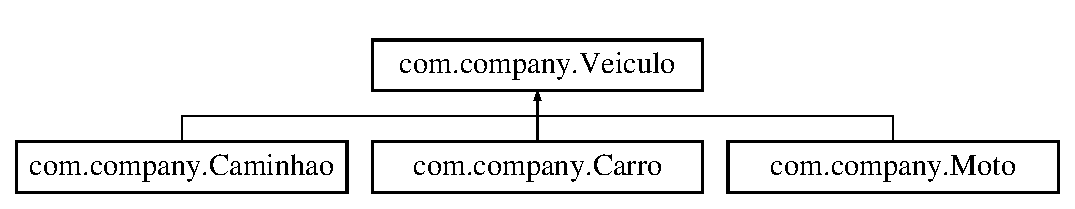
\includegraphics[height=2.000000cm]{classcom_1_1company_1_1_veiculo}
\end{center}
\end{figure}
\subsection*{Membros Públicos}
\begin{DoxyCompactItemize}
\item 
\mbox{\Hypertarget{classcom_1_1company_1_1_veiculo_af90053fd848a2af693c83745ddf8e1b2}\label{classcom_1_1company_1_1_veiculo_af90053fd848a2af693c83745ddf8e1b2}} 
\mbox{\hyperlink{classcom_1_1company_1_1_veiculo_af90053fd848a2af693c83745ddf8e1b2}{Veiculo}} ()
\begin{DoxyCompactList}\small\item\em inicia o veiculo com todos os privates zerados \end{DoxyCompactList}\item 
\mbox{\Hypertarget{classcom_1_1company_1_1_veiculo_a41c4df426c7a44865a91805033a90c40}\label{classcom_1_1company_1_1_veiculo_a41c4df426c7a44865a91805033a90c40}} 
\mbox{\hyperlink{classcom_1_1company_1_1_veiculo_a41c4df426c7a44865a91805033a90c40}{Veiculo}} (int xx, int yy, String modelo, int aux)
\begin{DoxyCompactList}\small\item\em inicia os veiculos ja com alguns privates iniciados e dado valores \end{DoxyCompactList}\item 
\mbox{\Hypertarget{classcom_1_1company_1_1_veiculo_aaa9b728af0c768d45303cf571fb87aad}\label{classcom_1_1company_1_1_veiculo_aaa9b728af0c768d45303cf571fb87aad}} 
int \mbox{\hyperlink{classcom_1_1company_1_1_veiculo_aaa9b728af0c768d45303cf571fb87aad}{getY}} ()
\begin{DoxyCompactList}\small\item\em retorna um valor para Y que no caso sera a posicao \end{DoxyCompactList}\item 
\mbox{\Hypertarget{classcom_1_1company_1_1_veiculo_a9ada153473ad718329e574b9d8b08303}\label{classcom_1_1company_1_1_veiculo_a9ada153473ad718329e574b9d8b08303}} 
void \mbox{\hyperlink{classcom_1_1company_1_1_veiculo_a9ada153473ad718329e574b9d8b08303}{setY}} (int p)
\begin{DoxyCompactList}\small\item\em salva um valor para Y que no caso sera a posicao \end{DoxyCompactList}\item 
\mbox{\Hypertarget{classcom_1_1company_1_1_veiculo_a1dc4509f0773ea671941bddf79ae7711}\label{classcom_1_1company_1_1_veiculo_a1dc4509f0773ea671941bddf79ae7711}} 
int \mbox{\hyperlink{classcom_1_1company_1_1_veiculo_a1dc4509f0773ea671941bddf79ae7711}{getX}} ()
\begin{DoxyCompactList}\small\item\em retorna um valor para X que no caso sera a posicao \end{DoxyCompactList}\item 
\mbox{\Hypertarget{classcom_1_1company_1_1_veiculo_aa2851a375fd6c1fce3a5ce9a91491fe5}\label{classcom_1_1company_1_1_veiculo_aa2851a375fd6c1fce3a5ce9a91491fe5}} 
void \mbox{\hyperlink{classcom_1_1company_1_1_veiculo_aa2851a375fd6c1fce3a5ce9a91491fe5}{setX}} (int p)
\begin{DoxyCompactList}\small\item\em salva um valor para X que no caso sera a posicao \end{DoxyCompactList}\item 
\mbox{\Hypertarget{classcom_1_1company_1_1_veiculo_a0dc8868a4af5688903e06f78876c44df}\label{classcom_1_1company_1_1_veiculo_a0dc8868a4af5688903e06f78876c44df}} 
void \mbox{\hyperlink{classcom_1_1company_1_1_veiculo_a0dc8868a4af5688903e06f78876c44df}{setX}} ()
\begin{DoxyCompactList}\small\item\em salva um valor para X que no caso sera a posicao porem aleatorio \end{DoxyCompactList}\item 
\mbox{\Hypertarget{classcom_1_1company_1_1_veiculo_ada176daedcc81fb7729b6e7628776905}\label{classcom_1_1company_1_1_veiculo_ada176daedcc81fb7729b6e7628776905}} 
void \mbox{\hyperlink{classcom_1_1company_1_1_veiculo_ada176daedcc81fb7729b6e7628776905}{setY}} ()
\begin{DoxyCompactList}\small\item\em salva um valor para Y que no caso sera a posicao posicao porem aleatorio \end{DoxyCompactList}\item 
\mbox{\Hypertarget{classcom_1_1company_1_1_veiculo_a2fdaf3ef088b809484f93f96753574dd}\label{classcom_1_1company_1_1_veiculo_a2fdaf3ef088b809484f93f96753574dd}} 
int \mbox{\hyperlink{classcom_1_1company_1_1_veiculo_a2fdaf3ef088b809484f93f96753574dd}{get\+Velocidade}} ()
\begin{DoxyCompactList}\small\item\em retorna a velocidade \end{DoxyCompactList}\item 
\mbox{\Hypertarget{classcom_1_1company_1_1_veiculo_a1e5cd5adf67832f217eb08b500a4a272}\label{classcom_1_1company_1_1_veiculo_a1e5cd5adf67832f217eb08b500a4a272}} 
void \mbox{\hyperlink{classcom_1_1company_1_1_veiculo_a1e5cd5adf67832f217eb08b500a4a272}{set\+Velocidade}} (int n)
\begin{DoxyCompactList}\small\item\em salva a velocidade \end{DoxyCompactList}\item 
\mbox{\Hypertarget{classcom_1_1company_1_1_veiculo_ac5031ed15eb034d06b31887f0965d690}\label{classcom_1_1company_1_1_veiculo_ac5031ed15eb034d06b31887f0965d690}} 
int \mbox{\hyperlink{classcom_1_1company_1_1_veiculo_ac5031ed15eb034d06b31887f0965d690}{get\+Posicao\+Antiga}} ()
\begin{DoxyCompactList}\small\item\em retorna a velocidade antiga \end{DoxyCompactList}\item 
\mbox{\Hypertarget{classcom_1_1company_1_1_veiculo_a01b02131f3f6956622443c9ae7e47e6e}\label{classcom_1_1company_1_1_veiculo_a01b02131f3f6956622443c9ae7e47e6e}} 
void \mbox{\hyperlink{classcom_1_1company_1_1_veiculo_a01b02131f3f6956622443c9ae7e47e6e}{set\+Posicao\+Antiga}} (int pn)
\begin{DoxyCompactList}\small\item\em salva a posicao antiga \end{DoxyCompactList}\end{DoxyCompactItemize}


A documentação para essa classe foi gerada a partir do seguinte arquivo\+:\begin{DoxyCompactItemize}
\item 
Veiculo.\+java\end{DoxyCompactItemize}

%--- End generated contents ---

% Index
\backmatter
\newpage
\phantomsection
\clearemptydoublepage
\addcontentsline{toc}{chapter}{Sumário}
\printindex

\end{document}
